\subsection{近似解的存在性}

给定数 \(\varepsilon > 0\)，我们称 I 到 H 中的连续映射 u 为下述微分方程精确到 \(\varepsilon\) 的近似解

\[
\mathbf {x} ^ {\prime} = \mathbf {f} (t, \mathbf {x})\tag{1}
\]

如果在 I 的一个可数子集的补集的所有点处，函数 u 都有满足下列条件的导数

\[
\left| \left| \mathbf {u} ^ {\prime} (t) - \mathbf {f} (t, \mathbf {u} (t)) \right| \right| \leqslant \varepsilon .\tag{7}
\]

设 \((t_{0}, \mathbf{x}_{0})\) 是 \(I \times H\) 的一点；由于 f 满足引理 1 的假设（IV，第 165 页），存在 \(t_{0}\) 在 I 中的紧邻域 J 使 \(\mathbf{f}(t, \mathbf{x}_{0})\) 在 J 上有界，又存在以 \(\mathbf{x}_{0}\) 为中心、包含于 H 中的开球 S，使 \(\mathbf{f}(t, \mathbf{x}) - \mathbf{f}(t, \mathbf{x}_{0})\) 在 \(J \times S\) 上有界；由此推出 \(\mathbf{f}(t, \mathbf{x})\) 在 \(J \times S\) 上有界。在本小节中，J 将表示 \(t_{0}\) 在 I 中的一个紧区间邻域，S 将表示以 \(\mathbf{x}_{0}\) 为中心、半径为 r 且包含于 H 中的开球，而 J 与 S 使得 f 在 \(J \times S\) 上有界；M 将表示 \(\| \mathbf{f}(t, \mathbf{x}) \|\) 在 \(J \times S\) 上的上确界。

命题 3. 在每个以 \(t_{0}\) 为左（或右）端点、包含于 J 中且长度小于 \(r/(M + \varepsilon)\) 的紧区间上，都存在方程 (1) 的精确到 \(\varepsilon\) 的近似解，其值属于 S，且在 \(x_{0}\) 处等于 \(t_{0}\)。

我们设 \(t_{0}\) 不是 J 的右端点，并对以 \(t_{0}\) 为左端点的区间证明本命题。设 M 为 (1) 的精确到 \(\varepsilon\) 的解所成的集，其中每个解取值于 S、在 \(x_{0}\) 处等于 \(t_{0}\)，并且定义在一个包含于 J 中的半开区间 \([t_{0}, b[\) 上（该区间随所考虑的近似解而异）。首先证明 M 非空。设 c 是 \(\mathbf{f}(t, \mathbf{x}_{0})\) 在 \(t_{0}\) 处的右极限；由引理 1（IV，第 165 页），函数 \(\mathbf{f}\big(t, \mathbf{x}_{0} + \mathbf{c}(t - t_{0})\big)\) 在 \(t_{0}\) 处有等于 c 的右极限，故函数 \(\mathbf{x}_{0} + \mathbf{c}(t - t_{0})\) 在足够小的半开区间 \([t_{0}, b[\) 上的限制属于 M。

我们用关系“u 是 v 的限制”给集合 M 排序，并证明 M 是归纳的（《集合论》，III，第 154 页）。设 \((\mathbf{u}_{\alpha})\) 是 M 的全序子集，\([t_{0}, b_{\alpha}[\) 是 \(u_{\alpha}\) 的定义区间：当 \(b_{\alpha} \leqslant b_{\beta}\) 时，函数 \(u_{\beta}\) 便是 \(u_{\alpha}\) 的扩张。诸区间 \([t_{0}, b_{\alpha}[\) 的并是一个包含于 J 中的区间 \([t_{0}, b[\)，并且存在唯一一个定义在 \([t_{0}, b[\) 上、与每个 \(u_{\alpha}\) 在 \([t_{0}, b_{\alpha}[\) 上都一致（对每个 \(\alpha\)）的函数 u；在诸 \(b_{\alpha}\) 中存在递增序列 \((b_{\alpha_{n}})\) 趋于 b；由于 u 在 \(u_{\alpha_{n}}\) 上与 \([t_{0}, b_{\alpha_{n}}[\) 一致，函数 u 在 \([t_{0}, b[,\) 的一个可数子集的补集的所有点处都有满足 (7) 的导数，因而它是集合 \((\mathbf{u}_{\alpha})\) 在 M 中的上确界。

由佐恩引理（《集合论》，III，第 154 页，定理 2），\(\mathfrak{M}\) 有一个极大元 \(\mathbf{u}_0\)；我们将证明：若 \([t_0, t_1[\) 是 \(\mathbf{u}_0\) 的定义区间，则或者 \(t_1\) 是 J 的右端点，或者 \(t_1 - t_0 \geqslant r / (\mathbf{M} + \varepsilon)\)。我们用反证法，假设这两个条件都不成立；首先证明可以把 \(\mathbf{u}_0\) 连续地延拓到点 \(t_1\) 处；事实上，对任意 \(s\) 与 \(t\)（属于 \([t_0, t_1[\)），

\[
\left\| \mathbf {u} _ {0} (s) - \mathbf {u} _ {0} (t) \right\| \leqslant (\mathrm{M} + \varepsilon) | s - t |
\]

这是依中值定理得到的；柯西准则表明 \(\mathbf{u}_0\) 有左极限 \(\mathbf{x}_1 \in S\) 于点 \(t_1\)。现设 \(\mathbf{c}_1\) 是函数 \(t_1\) 在 \(\mathbf{f}(t, \mathbf{x}_1)\) 处的右极限；有 \(\| \mathbf{c}_1 \| \leqslant M\)；与证明开头同样的论证表明，可以把 \(\mathbf{u}_0\) 延拓到一个以 \(t_1\) 为左端点的半开区间上，延拓所用的函数是 \(\mathbf{x}_1 + \mathbf{c}_1 (t - t_1)\)，从而延拓后的函数属于 \(\mathfrak{M}\)，这是荒谬的。这就证明了本命题。

当 \(\mathbf{f}\) 在 \(\mathrm{J} \times \mathrm{S}\) 上一致连续时，可以不用佐恩引理来证明命题 3（IV，第 199 页，习题 1a)）。

命题 4. (1) 的精确到 \(\varepsilon\) 、定义在同一区间 \(K \subset J\) 上且取值于 S 中的近似解所成之集是一致等度连续的。

的确，若 \(\mathbf{u}\) 是这个集中的任一函数，而 \(s\) 与 \(t\) 是 \(\mathbf{K}\) 的两个点，则由中值定理

\[
\left\| \mathbf {u} (s) - \mathbf {u} (t) \right\| \leqslant (\mathrm{M} + \varepsilon) | s - t |.
\]

推论（佩亚诺定理）. 若 E 在 R 上是有限维的，则存在 (1) 的一个解，其值属于 S，且等于 \(x_{0}\) 于 \(t_{0}\)，这里 K 是任一以 \(t_{0}\) 为左（或右）端点、包含于 J 中且长度 \textless{} r/M 的紧区间。

的确，由命题 3，一旦 \(n\) 足够大，就存在 (1) 的近似解 \(\mathbf{u}_n\)，其精确度为 \(1/n\)，它定义在 \(\mathbf{K}\) 上，取值于 \(\mathbf{S}\) 中，且在 \(\mathbf{x}_0\) 处等于 \(t_0\)。此外，从 \(n\) 的某个值起，\(\mathbf{u}_n(\mathbf{K})\) 包含在一个以 \(\mathbf{x}_0\) 为中心、以 \(< r\) 为半径（与 \(n\) 无关）的闭球中。诸 \(\mathbf{u}_n\) 所成之集是等度连续的（命题 4），又因 \(\mathbf{E}\) 是有限维的，集合 \(\mathbf{S}\) 在 \(\mathbf{E}\) 中相对紧；于是对每个 \(t \in \mathbf{K}\)，诸 \(\mathbf{u}_n(t)\) 所成之集在 \(\mathbf{E}\) 中相对紧。由阿斯科利定理（《一般拓扑学》，X，第 290 页，定理 2），诸 \(\mathbf{u}_n\) 所成之集在由 \(\mathcal{F}(\mathbf{K};\mathbf{E})\) 到 \(\mathbf{K}\) 中的映射所组成、赋有一致范数的空间 \(\mathbf{E}\) 中相对紧。于是存在序列 \((\mathbf{u}_{n_k})\)，它是从 \((\mathbf{u}_n)\) 中抽取出来的，并且在 \(\mathbf{K}\) 上一致收敛于某个连续函数 \(\mathbf{u}\)。我们有 \(\mathbf{u}(\mathbf{K}) \subset \mathbf{S}\)，故 \(t \mapsto \mathbf{f}(t,\mathbf{u}(t))\) 在 \(\mathbf{K}\) 上有定义；由引理 1（IV，第 165 页），\(\mathbf{f}(t,\mathbf{u}_{n_k}(t))\) 一致收敛于 \(\mathbf{f}(t,\mathbf{u}(t))\)（在 \(\mathbf{K}\) 上）；由（IV，第 4 页，公式 (7)），\(\mathbf{u}_{n_k}\) 是某个一致趋于 \(\mathbf{f}(t,\mathbf{u}(t))\)（在 \(\mathbf{K}\) 上的）函数的原函数，故（II，第 52 页，定理 1）\(\mathbf{u}\) 是 (1) 在 \(\mathbf{K}\) 上的解，且在点 \(\mathbf{x}_0\) 处等于 \(t_0\)。

\pandocbounded{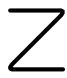
\includegraphics[keepaspectratio]{images/part001_11d71cd9.jpg}}

注. 1) 一个微分方程 (1) 在给定点处取同一值的积分可以有无穷多个。例如，数量微分方程 \(x' = 2\sqrt{|x|}\) 以由下列式子定义的诸函数

\[
\begin{array}{l l} u (t) = 0 & \text { for } \quad - \beta \leqslant t \leqslant \alpha \\ u (t) = - (t + \beta) ^ {2} & \text { for } \quad t \leqslant - \beta \\ u (t) = (t - \alpha) ^ {2} & \text { for } \quad t \geqslant \alpha \end{array}
\]

为其在点 t = 0 处取值 0 的积分，这里 \(\alpha\) 与 \(\beta\) 为任意正数。

\begin{enumerate}
\def\labelenumi{\arabic{enumi})}
\setcounter{enumi}{1}
\tightlist
\item
  当 \(\mathbf{E}\) 是任意无穷维的完备赋范空间时，佩亚诺定理不再成立（IV，第 204 页，习题 18）。
\end{enumerate}

